\section{Fordeling af besvarelserne}
\label{TestAfSkalaFordeling}
%
(her skrives om normalfordeling og historgrammer)

(her skrives om boksplottet ift skalaerne)

\subsection{Varians}
%
For at få et overblik over hvor meget besvarelserne variere og hvor stor forskel der er mellem variationen ved de forskellige SQ, beregnes variansen for hver SQ beregnes med formlen: \blankline
%
\begin{equation}
	Var = \frac{\sum_{i=1}^{n}(x_i-\overline{x})^{2}}{(n-1)}
\end{equation}
\noindent
%
\fxnote{Indsæt kilde (Field bog)}
Hvor $Var$ er varians, $x_i$ er målingen for nummer $i$, $\overline{x}$ er middelværdien og $n$ er antal målinger. 
En oversigt over variansen for hver SQ kan ses på \autoref{fig:Varians}. 
%
\begin{figure}[H]
\centering
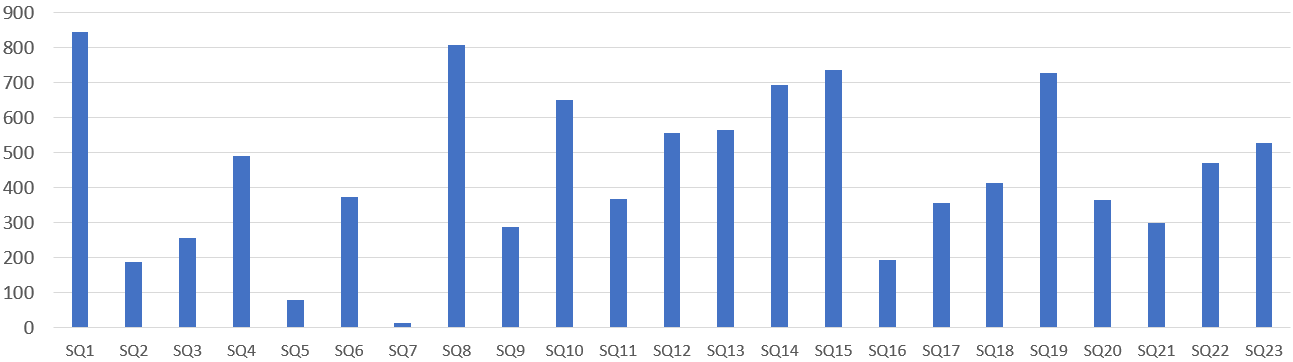
\includegraphics[width = \textwidth]{Figure/DatabehandlingSkalaer/Varians} 
\caption{Søjlediagram over variansen for besvarelserne til hvert Scale Question.}
\label{fig:Varians}
\end{figure}
\noindent
%
Det tydeligt at se ud fra \autoref{fig:Varians} at der er stor forskel mellem variansen ved de forskellige SQ. For eksempel er variansen for SQ5 og SQ7 meget lav i forhold til SQ1 og SQ8. 
%
\subsection{Standardisering af besvarelser}
Når variansen ikke er ens for ens data kan det i nogle tilfælde vælges at udligne variansen. Hvis variansen skulle udlignes vil der skulle laves en standardisering af data. Formålet med at gøre dette er at data med lav varians i rå data får lige betydning i PCA som rå data med stor varians. \blankline
%
Det vælges ikke at standardisere data, da det kan give skævvridninger som ikke er ønsket. Testpersonerne har reelt haft muligheden for at besvarer på hele skalaen, men har valgt at give besvarelser i nærheden af hinanden, hvilket tolkes som at de har været mere enige i dette tilfælde. \blankline
%
Al data er målt med samme måleenhed, da det er målt på samme skala, der går fra 0 til 100 ved aflæsningen. Dette er en del af begrundelsen for ikke at standardisere, da det ofte gøre i tilfælde hvor målingerne ikke er målt med samme måleenhed. \blankline
%
Hvis der er større variation ved nogle skalabesvarelser, vil de vægte mere i en PCA, men det vurderes at være acceptabelt og ønsket. Det er dog vigtigt at være opmærksom på dette, når resultaterne af PCA analyseres. 
